\chapter{Project Overview}

Socneto is a framework for analysing data from social networks for a given topic. Socneto can be extended with custom data acquirers and custom analyser. Socneto supports two major social networks: Twitter\footnote{\url{www.twitter.com}} and Reddit\footnote{\url{www.reddit.com}}; and two data analysers of key topics and sentiment supported in the current version of Socneto. 

% \todo{Možná bych (i jidne v textu) zdůraznila, že ty dvě SN a analyzátory jsou podporované v aktuální verzi SW, ale je možné přidávat další. Obecně tu rozšiřitelnost je potřeba vhodně zdůraznit.} 

\section{Introduction}\label{section:intro}

This chapter opens with Section \ref{section:problemAnalysis} which introduces the problem that Socneto tackles. The following Section \ref{section:relatedWork} then compares Socneto with products focusing on either social networks or data processing. Section \ref{section:realuc} describes achievements of the Socneto in the real world. At the end of this chapter, Section \ref{section:timeline} traces the project development process. 

\section{Problem Analysis}\label{section:problemAnalysis}
% Stručné uvedení do problematiky, kterou projekt řeší

This section introduces what solution Socneto offers to the major problems concerning social networks and data analysis tools. Each of the problem and its solution is discussed separately. The problems are the following:

\begin{itemize}
    \item A content personalization
    \item Abundance of data
    \item Social networks API limits
    \item Limited customization
\end{itemize}

\subsection{A Content Personalization}
% - Not from one source (influencer or whatever) - from topic to people and related topics, not the other way arround

Social networks, such as Twitter and Reddit, allows users to easily subscribe to a content producer or to a group interested in some topic. This personalization may result in the user being enclosed in a bubble without being confronted with the opposite view. User is not exposed to anything that does not fall into user's field interest. It makes it easy for the content producers to influence their subscribers (hence the word influencers).

Socneto solves this problem by inverting the approach to the content searching. As stated above, users usually follow influencers or groups that publish posts related to some topic. The opposite approach, which is implemented in Socneto, is to search for a topic and find the content creators and other related topics.

% problem of too much data
\subsection{Abundance of Data}

The other problem social networks posses is the large amount of data that is not possible to read through them all and make one's opinion. Social networks do not typically offer a tool helping the user to improve orientation in the vast amount of data with comprehensive statistics of related topics, sentiment and such.

All data downloaded are accessible to the users to visualize their properties with various charts. The user can see a number of posts related to the given topic on the timeline, sentiment development in the time, top related topics.

% api limits
\subsection{API Limits}

Although social networks have their data publicly accessible, it is not an easy task to access it. Access to the data via API is limited in two ways. One way is a limit imposed on a number of posts that can be downloaded per a given time period (typically 15 minutes or an hour).  The other limit is imposed on the latest post which can be downloaded. For example the latest accessible post is only a week old which makes it impossible to analyse post of the past. (The limits are discussed in Chapter Implementation, Section \ref{section:acquirers}) 

Socneto overcomes the API limits by downloading the data continuously over a long period of time utilizing the limits to its maximum. It does not help users who want to analyse the history of the topic, but it helps people who know the topic in advance. When such user submits a job and the data starts flowing, the results can be seen immediately - Socneto is designed to calculate the analyses on the fly so the user always has the data up-to-date.

% Customizable working pipeline
% limited capabilites

\subsection{Limited Customization}

% this should be revisited and rewritten to make more sense.
There are various tools that focus on either downloading or analysing (or both) data from social networks (for deeper analysis refer to Section \ref{section:relatedWork}). These tools are either full fledged services that are not customizable at all or, on the other hand, the tool is an open source script that is customizable but typically is focused only on analysis or acquisition therefore it lacks functionality.

Socneto finds the middle ground by allowing users to add support for social network data acquisition and analysis out of the box as long as the components follow basic component life cycle and interfaces(for more details refer to Chapter \ref{chapter:extensibility}). When the users submit a job they can select multiple acquirers and analysers and also customize result visualizations.

% Zasazení vytvořeného díla do kontextu existujících programových děl řešících obdobnou problematiku
% - https://monitora.cz/
% - Sphere
% - Spark + data processing appraoch

%  - kategorie
%  - shrnuti vyhod a nevyhod

\section{Related Works}\label{section:relatedWork}

Socneto combines three major fields of interest: social networks, data processing and data analysis. Although there are plenty of tools and services that cover at least one of the fields, this section mentions only those that cover two or all three.

\subsection{Field of Interest Classification}

\subsubsection{Social Networks}

Social networks\footnote{YouTube and Reddit are also considered social networks in this text} are used by many types of users with various needs and requirements. The majority of the users are people that mostly consume the content and occasionally share something with friends or followers. The types of users that focus more on producing are companies or public bodies. While typical consuming users expect to have easy access to the content creators, the needs of the producers are more elaborate and can be summarized as follows:

\begin{itemize}
    \item Intelligence - watching out for trends, consumer needs and profile appeal
    \item Influence Statistics - monitoring of posts influence
    \item Social Customer Care - swift reaction to posts or comments
    \item Social Media Management - publishing management and approval process and
\end{itemize}



\subsubsection{Web monitoring and analysis}

Data processing framework is expected to process and save large amounts from various sources of data of various types and shapes. The most notable properties of data processing framework are:

\begin{itemize}
    \item Multisource - Monitoring of data from various sources. 
    \item Multicontent - Ability to process textual, visual, audio and audiovisual material.
    \item Reporting - Comprehensive data presentation
\end{itemize}

In this context, data analysis is understood as a function of a tool to extract useful information from incoming data. Since Socneto analyses only textual data, the types of analyses that work with non-textual data are omitted in the following text. The tools falling into this category range from trivial functions such as word counters to very complex methods employing machine learning, such as sentiment analysis.

\subsubsection{Competitors}

This section introduces four competitors falling into two categories according to their primary focus. The list of competitors is not exhaustive. The competitors merely are representing their category. The categories along with their representatives are the following:

\begin{itemize}
    \item Social Network - Zoom Sphere\footnote{\url{www.zoomsphere.com}}, Social Bakers\footnote{\url{www.socialbakers.com}}
    \item Web Monitoring and Data Analysis - Monitora\footnote{\url{Monitora}}, Google Flu Trends\footnote{\url{https://www.google.org/flutrends/about/}}
\end{itemize}

%\paragraph{Primary Focus: Social networks}


\paragraph{ZoomSphere}
% \todo{Každý ten tool by tady mohl mít screen shot pro představu - ale nemusí.}
A tool focusing primarily on presentation and brand management is Zoom Sphere whose goal is to help companies or influencers to thrive on the supported social networks. Both products offer an extensive analysis of a current brand status focused on measuring the impact of created posts.

\paragraph{Social Bakers}

One of the best services in the market is Social Bakers offering a solution to the majority of problems stemming from managing social networks. According to its web page, it fulfills all the requirements discussed in social networks classification. Customers' needs are monitored on various levels ranging from conversational level -- hot topic classification -- to high-level brand sentiment. 

% todo add argument to the other facets of good social network tool

%\paragraph{Primary Focus: Web Monitoring and analysis}

\paragraph{Monitora}

Full-fledged media monitoring tools represented by Monitora that not only scrapes but also analyses and aggregates the scraped data. While the former tool is used by tech-savvy users who want only some data, the latter is a paid service that is claimed to employ a team of specialists to collect and interpret the results. This service is used by customers wishing to be informed public opinion.

\paragraph{Google Flu Trends}

Another service keeping track of web content is recently shutdown service Google Flu Trends which monitored Google Search activity related to searches of influenza. Such searches were used to predict the start of a ``flu season'' in more than 25 countries. 

\subsubsection{Comparison}

In this section, Socneto is compared to the above-mentioned products. The main criteria are the following:

\begin{itemize}
    \item Integration with social networks - Ability to connect to a social network and utilize its features.
    \item Searching capabilities - Ability to search continuously for the topic of interest across the web.
    \item Analysis and reporting - Ability to extract and present information from a vast amount of data.
    \item Extensibility - Ability to add user specific functionality
\end{itemize}

\paragraph{Integration with Social Networks}

The best integration with social networks is offered by Social Bakers which offers the best suite to utilize social network features. It connects content from all large social networks (such as Facebook, Twitter, LinkedIn\footnote{\url{www.linkedin.com}}) and services that users use to consume and comment on the content such as YouTube\footnote{\url{www.youtube.com}}. Similarly to Social Bakers, ZoomSphere offers similar features. Both applications offer many charts that the user can easily set up and personalize and both require the user to explicitly connect the application with a profile.

Monitora does not have such requirements and offers similar reporting features related to social networks. Monitora is not restricted to social networks, it can scrape any important source of information on the internet. Lastly, Google Flu Service does not work with social networks at all. 

\paragraph{Searching Capabilities}

The broadest searching capabilities are offered by Monitora whose data sources include Radio Broadcast, TV, press and online content (social networks included)\footnote{\url{https://monitora.cz/monitoring-medii/}}. On the top of that, Monitora archives the content and up to now offers content from the past 20 years. Therefore Monitora excels in the variety of data it covers and in its continuous acquisition. On the other hand, Google Flu trends utilize only Google Search input but it has access to the history of all Google searches.

The data sources of Zoom Sphere and Social Bakers are limited only to social networks. They archive all the data related to the given user profiles and also continuously monitor all related data. 

\paragraph{Analysis and reporting}

Zoom Sphere\footnote{\url{https://www.zoomsphere.com/analytics}} and Social Bakers\footnote{\url{https://www.socialbakers.com/solution/measurement-and-reporting}} analytic tools focus primarily on metrics important to a social network user such as the impact of a post or the trend analysis so the user can create posts with the best possible influence. Both Zoom Sphere and Social Bakers offer a variety of reporting tools to visualize all the data. Monitora\footnote{\url{https://monitora.cz/analyza-medii/}} offers similar types of analyses and reports without limiting itself to social networks only. Google Flu Trends is an analytic tool itself.

\paragraph{Extensibility} 

Zoom Sphere does not explicitly offer any means of extensibility they are covering most of the required functionality of the social network domain out of the box. Social Bakers have a similar approach, yet the platform can be extended but the customer would have to participate in the partnership program\footnote{\url{https://www.socialbakers.com/integrations-and-partnerships}}. Monitora is not an extensible product, but its creators offer custom services\footnote{\url{https://monitora.cz/kontakt/\#sluzby}}. 

Google Flu Trends offered their API for users to potentially implement custom analysis on the top of the google search data. Although the service was closed in August 2015 \footnote{\url{https://www.google.org/flutrends/about/}} and the API is no longer available, the datasets are available for academic purposes.

\paragraph{Comparison with Socneto}

In terms of social network capabilities, Socneto is not a competitor to Social Bakers or Zoom Sphere. Especially with the user-profile oriented capabilities. These two products focus on a user profile (or multiple profiles at once) and analyse only data related to its activity. Socneto, on the other hand, works the other way round. It searches for any information relevant to a given topic regardless the user profile which is the similar approach Monitora implements.

The searching capabilities of Socneto that are supported in the current version (further extensible) is limited to Reddit and Twitter only. The strong point is that these social networks are monitored continuously and data are also stored in an archive. 

The supported analyses of the current version of Socneto correspond to the way Socneto obtains data. The analyses are applied to the data for the given topic producing public opinion through sentiment analysis or related topics through topic modeling (see Chapter \ref{chapter:analysis}). Given the fact that Socneto does not focus on a particular user or a profile, the post-specific analyses could not be implemented. But with the proper prediction model, Socneto can be easily extended to simulate Google Flu Trends, but applied to social networks.

The products that were discussed in this section lack the ability to easily extend their functionality in which Socneto stands out. Socneto has the potential to compete with the other through extensibility (see Chapter \ref{chapter:extensibility}) in the following way:

\begin{itemize}
    \item Zoom Sphere and Social Bakers - Both products excel in the integration with social networks and in the focus on a profile rather than a broad overview. Although Socneto already implements social network data acquisition, it can implement another one which does not search through data related to the given topic but focus on all data related to a single user.
    \item Monitora - The strongest side of Monitora is the broad scope of sources it can track. Socneto's collection of data sources does not have to be limited to social networks or textual data.
    \item Google Flu Trends - The flu prediction can be incorporated into Socneto Analysis and then applied on the data from various other sources.
\end{itemize}

In conclusion, Socneto has a great potential to compete on the market. In its current form, Socneto can be understood as a flexible framework that can be modified to serve multiple purposes.  

% - Add usecases of our users
%  - MSF
%  - CES
%  - Reddit academics
\section{Real-World Use Cases}\label{section:realuc}

Socneto helped to get a grasp of social network data in the following two cases:

\begin{itemize}
    \item Doctors without Borders\footnote{\url{https://www.lekari-bez-hranic.cz/}} - analysis of measles and snake bites.
    \item Datamole\footnote{\url{https://www.datamole.cz/}} - summarizing most discussed topics Consumer Electronic Show (CES)\footnote{\url{www.ces.tech}} on Twitter
\end{itemize}

\subsection{Measles and Snake Bite Analysis}

Doctors without Borders, represented by Jan Böhm whose responsibility, among others, is studying and monitoring social networks. Socneto was used for analysis of topics related to two given ones: measles and snakebites. The analysis consisted of running two separate jobs for each topic and gathering data for a period of 40 days. 

As stated by Jan Böhm, the results showed several ``interesting remarks that can be used in their work''  and also revealed limits of the easily accessible Twitter tweets and their misleading nature. Although the query was given in three languages: English, French and Arabic, the results were mostly in English (as can be seen in Figure \ref{figure:msf_lang}). According to Jan Böhm, "this supports a theory that Twitter is mainly used as a tool for reporting the news to the world and not for communication among locals whereas Facebook is claimed to be the platform for such purpose". 

\begin{figure}
    \centering
    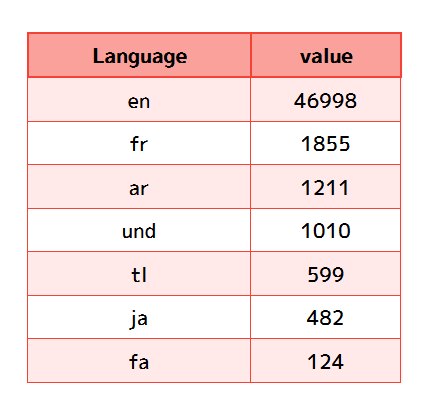
\includegraphics[scale=0.7]{diagrams/po_msf_lang.png}
    \caption{The graph show distribution of languages for a query \texttt{measles} in French, Arabic and English}
    \label{figure:msf_lang}
\end{figure}

The next occasion where Socneto proved itself was an analysis of trending topics of a convention Consumer Electronic Show (CES)\footnote{\url{https://www.ces.tech/}} that took place at the beginning of January 2020. Socneto helped to get a grasp of 120 thousand tweets during the three-day convention. The related topic analysis revealed that the most discussed topics were related to the television and car industry.

% no feedback will be present

% chronologický popis průběhu prací na projektu
% - Idea crystaliziation
% - First poc
% - Find real world users
% - finish
% - show
% - defend
% - party

\section{Project Timeline}\label{section:timeline}

The diagram of the project timeline is shown in Figure \ref{img:timeline}. The following text follows its structure.

\begin{figure}[h]
  \centering
    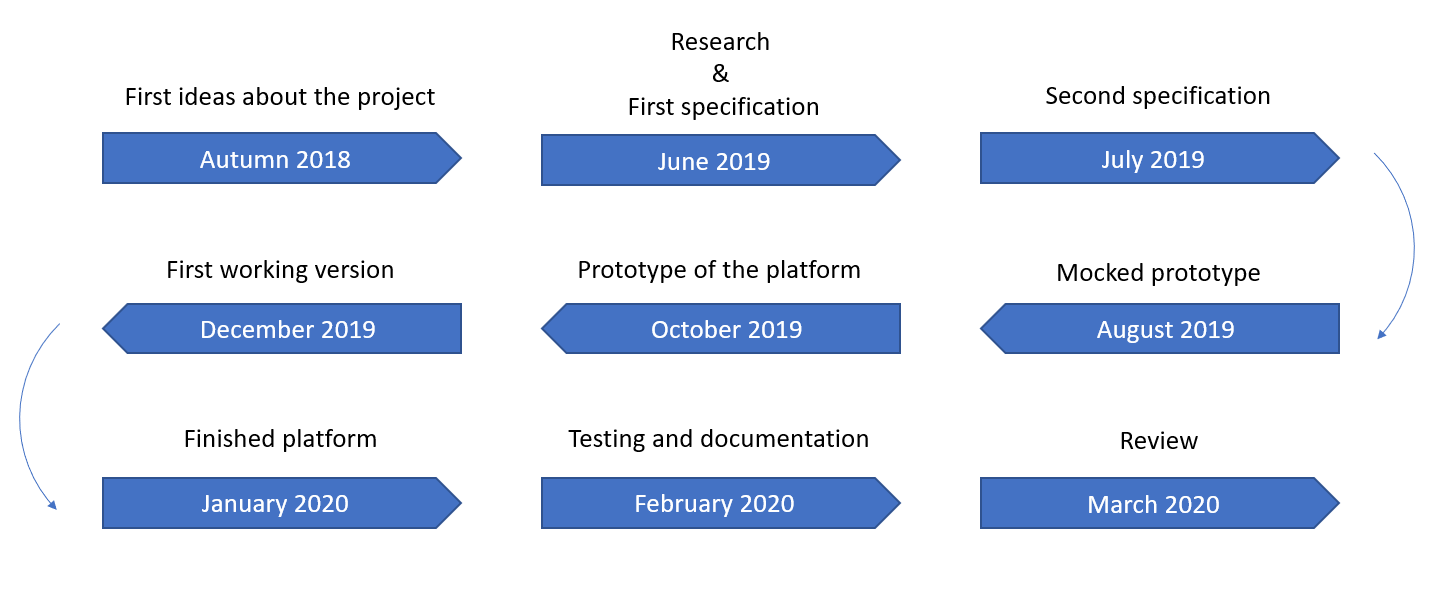
\includegraphics[width=\textwidth]{diagrams/timeline.png}
        \caption{Socneto development timeline showing the progress since Autumn 2018}
        \label{img:timeline}
\end{figure}

\subsection{Autumn 2018 - The First Idea}

The idea of creating a framework for data processing can be traced to Autumn 2018 and was motivated by the lack of practise with a big data framework. This idea was then consulted with the supervisor Doc. RNDr. Irena Holubová, Ph.D. who offered various feedback and helped us to find companies interested in cooperation. No cooperation was considered feasible though.  Soon after, Jan Pavlovský (a former member of the team) came up with an idea to focus on social network analysis. The idea seems to be interested enough for both parties and the search for the member started. Each member joining the team came up with ideas and the project started to take more solid shape. After many discussions, we came up with the idea of Socneto in June 2019 and the official project could start. 

\subsection{June 2019 - Official Start}
The software project work opened with writing the short specification with all the important ideas and features of the upcoming project. After it was accepted, the work on the second, full, specification could start. This document should contain not only a technical overview but also insight into project direction and management. We had an idea of separating the development into three stages: 
\begin{itemize}
    \item proof-of-concept - a project exploring the playing field, 
    \item full application - first application with all working components
    \item testing and documentation - last stage of the development
\end{itemize}

\subsection{July 2019 - Proof-of-Concept and Full Specification}

The proof of concept was finished along with the full specification in July 2019. At the time we were quite confident that we will not encounter any blind alley that would prevent us from finishing the project. Although most of the smart components were mocked, we found out that an application featuring an asynchronous messaging system would work. All mocked components were able to communicate well and others can be plugged in easily. 

\subsection{August 2019 to December 2019 - Working Prototype}

Most of our effort was put into replacing mocked components with working ones. Jaroslav Knotek finalized components downloading data from Twitter and Reddit. On top of that, we also added a component for the custom dataset which helped us with testing and at the end, it is a valuable addition to the offered ``data acquirers'' (for more information, see guide walking a user through the usage of custom dataset in Chapter \ref{chapter:extensibility}). 

Petra Vysušilová worked on sentiment analysis and topic modeling, replacing simple models with more elaborate ones. For better results, it was essential to get a more powerful infrastructure used for the training. For this purpose, the university GPU cluster was used to help train the model in a reasonable time. 

The entity model and all storage capabilities of Socneto were developed by Lukáš Kolek who built up storage for posts, their analysis, and all metadata. His part of Socneto, the whole database layer, is used by most of the components and is crucial for its proper function. Lukáš also helped to design interfaces between components so the communication would be as smooth as possible. 

The most visible part of the application was designed and implemented by Jůlius Flimmel who made it possible to visualize analyses and thus made them easily accessible. He was also responsible for designing the backend part of Socneto to ensure correct integration with the frontend.

This period was the time when Jan Pavlovský left the team after mutual agreement. Jan helped us the most at the beginning of the project when he proved to be a constant source of ideas. In the later phases, he has contributed to the architecture and a visual appearance. Unfortunately, his interest in the project was gradually diminishing after a discussion it was clear that did not intend to keep pace with the team. The project continued on with few changes. The support for the Czech language was omitted and all requirements concerning machine learning activities were lowered since Petra was the only remaining member capable of performing the task diligently.

\subsection{January 2020}

Because of a careful planning at the beginning, the implementation phase went smoothly without major hiccups. At the end of  December, we had a working platform with all the necessary components. It was time to find real-world users. With the help of Jiři Suchomel from the PR Department of the Faculty of Mathematics and Physics, we met Jan Böhm for whom we successfully analysed Twitter posts concerning measles and snake bites (for more details, see Section \ref{section:realuc}). 

\subsection{February 2020}
At the beginning of 2020 with the platform finished, we could start proper testing and documenting. At that time, we wrote scripts that start only a selected component in a controlled environment and assert its behaviour (see Chapter \ref{chapter:testing}). The documentation was written mostly during February. The 1st of March 2020 is the final deadline and according to the Software Project Committee customs we would be finished with defense by the end of the march. 